\documentclass[11pt, fleqn]{article}
\usepackage[a4paper, margin=2.54cm]{geometry}
\usepackage[utf8]{inputenc}
\usepackage[spanish, mexico]{babel}
\usepackage[spanish]{layout}
\usepackage[article]{ragged2e}
\usepackage{textcomp}
\usepackage{amsmath}
\usepackage{amssymb}
\usepackage{amsfonts}
\usepackage{graphicx}
% \usepackage{proof}

\setlength{\parindent}{5pt}

\title{%
    Trabajo Práctico N° 1 \\
    \large Teoría de Bases de Datos}
\author{Díaz, Agustín \and Farizano, Juan Ignacio \and Mellino, Natalia} %% faltan poner los legajos
\date{}

\begin{document}
\maketitle
\noindent\rule{\textwidth}{1pt}

\section*{Ejercicio 1}

Realizamos el Diagrama Entidad-Relación para el problema dado bajo los siguientes supuestos: 

\begin{itemize} % fari arregla las comillas que quedan feas
    \item La entidad Zona no tiene atributos suficientes para ser una entidad fuerte
          ya que su atributo nombre puede ser compartido por otras zonas. Por lo tanto, 
          la clasificamos como una entidad débil que depende de la entidad fuerte Población.
    \item Los clientes, vendedores y propietarios son identificados mediante un código de persona
          por lo tanto decidimos hacer una generalización de las entidades
          Cliente, Vendedor y Propietario con la entidad Persona.
    \item Las características de los inmuebles poseen atributos suficientes como para conformar una
          entidad fuerte, por lo tanto la misma será una entidad y no un atributo de la entidad Inmueble. 
\end{itemize}

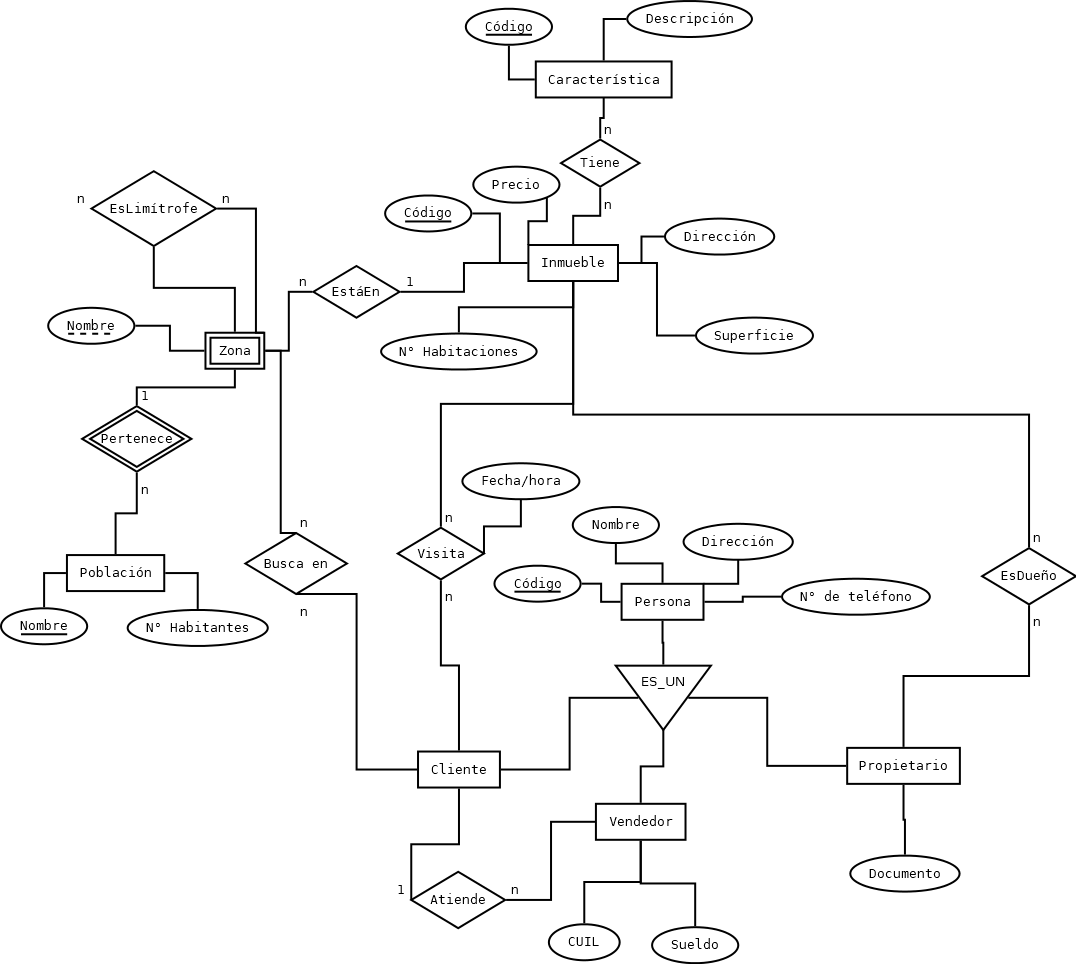
\includegraphics[width=15cm, height=12cm]{DER.png}

\end{document}